\chapter{Evaluation of Algorithmic Methods}
The optimisation of dielectric resonator shape and size within MASER systems is
a novel area of research, with no established methodologies in literature.
Traditional MASER resonator designs tend to rely on standardised geometries such
as toroids using squares or cylinders. This project aimed to explore a much
roader design space, where the resonator geometry could be modified in complex
and potentially non-intuitive ways to maximise performance. Given this
objective, it was necessary to first evaluate a wide range of potential
modelling strategies.

Due to the inherent axisymmetric structure of MASER cavities and to reduce
computational cost, all resonator geometries in this project were modelled using
COMSOL's 2D axisymmetric mode. This simplification assumes cylindrical symmetry
around a central axis, which not only halves the dimensional complexity of the
problem but also significantly reduces memory usage and simulation time. Figure
\ref{fig:figure6} shows a 3D cross-section of a typical MASER, with a zoomed-in
view of the 2D axisymmetric section used for simulation in COMSOL. This 2D slice
represents the effective modelling domain, capturing the radial and vertical
structure of the cavity. This unfortunately means that geometries with asymmetry
or complex 3D features are unable to be modelled in this project. However, 3D
modelling in possible in COMSOL (and many other electromagnetic simulation
tools) so there is the possibility of exploring this in future.

\begin{figure}[htbp]
  \centering
  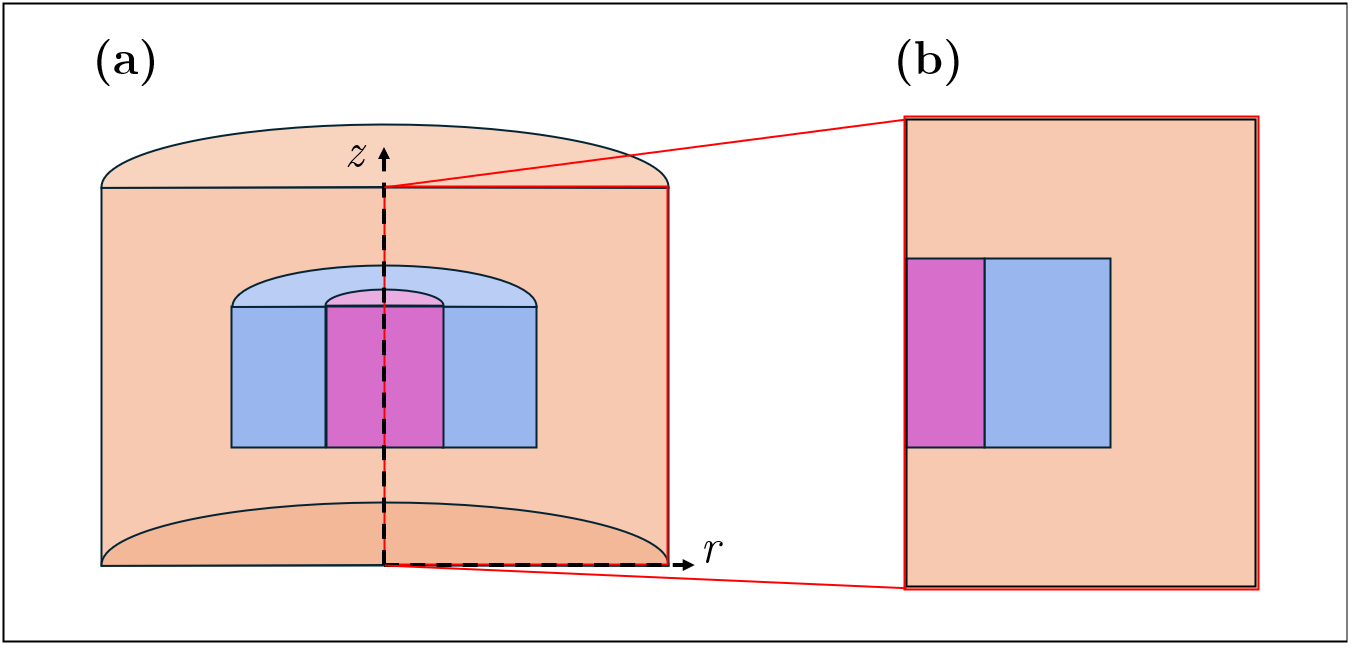
\includegraphics[width=0.7\textwidth]{figures/figure6.png}
  \caption{
    (a) 3D schematic of a typical MASER cavity showing the cylindrical symmetry
    of the structure. (b) Zoomed-in cross-section illustrating the 2D
    axisymmetric view used for COMSOL modelling, where only the $r$-$z$ plane is
    simulated.
  }
  \label{fig:figure6}
\end{figure}

All these models face the challenge of retaining the resonant frequency of 1.45
GHz. Scaling the global geometries either up or down depending on whether the
frequency is too high or low is the simplest way to fix this problem. However,
upon implementation into an optimisation algorithm that needs to run concurrent
simulation, the model will need to be ‘remeshed’ every time, greatly increasing
computational cost. To avoid this the global permittivity values (for both the
dielectric and air) can be scaled by a factor, $\alpha$. This is equivalent to
scaling the geometry but without the need to remesh.

This section reviews the main modelling strategies that were considered at the
outset of the project.

\section{The Slice Method}
\label{sec:section7}
In the first and simplest method, the inner wall of the dielectric resonator is
constrained to follow the vertical outer boundary of the gain medium. This
vertical line, defined over a prescribed axial interval, serves as a static
inner contour. From a set of evenly spaced points along this vertical line,
horizontal radial lines are projected outward. Each of these horizontal segments
has a tunable length $r_i$, which determines the radial extent of the resonator
at a given height. Connecting the endpoints of these vectors produces a
continuous 2D shape representing the cross-section of the dielectric resonator.
This is visually represented in Figure \ref{fig:figure7}(a).

Despite being simple and having good granularity control (by simply increasing
the number of horizontal segments), this method was ultimately not selected for
final optimisation due to its inability to represent irregular shapes, such as
dielectrics with overhangs or undercuts.

\section{The Polygon Method}
\label{sec:section8}
In this approach, the shape of the dielectric resonator is defined by a set of
discrete vertices, each located within the spatial boundaries set by the cavity
walls and the fixed gain medium. Each vertex is described by its cylindrical
coordinate pair ($r_i$, $z_i$), allowing complete geometric freedom within the
permitted design region. These points are then connected sequentially; each
point joined to its neighbours to form a closed, continuous 2D shape. This
method is shown in Figure \ref{fig:figure7}(b).

This approach offers maximal flexibility, as it does not assume any underlying
symmetry or regular structure in the resonator. However, this method introduces
several computational challenges. Firstly, the lack of inherent symmetry results
in greater mesh complexity and longer simulation times in COMSOL. Secondly,
maintaining a valid, non-self-intersecting polygonal structure during
optimisation requires additional geometric constraints. Therefore, this method
was rejected for final optimisation implementation.

\section{The Amoeba Method}
\label{sec:section9}
The geometry is defined by a central point, aligned with the axis of symmetry
in a cylindrical coordinate system. From this centre, a dense set of vectors is
projected outward, each characterised by a length $r_i$ and an angle $\theta_i$
from the horizontal axis. A sufficiently large number of these vectors
(typically 50 or more) are used such that the connected endpoints form a closed
curve with a high degree of smoothness. The result is shown in Figure
\ref{fig:figure7}(c) and resembles the contours of an amoeba, hence the name.

This approach offers a highly flexible parameter space, enabling the
representation of complex, asymmetric geometries that may not be accessible
through more rigid section- or grid-based methods. This method could also be
combined with spline interpolation to further smooth the contour[67]. Despite
its flexibility, it is unable to produce geometries with self-intersections or
internal vacancies as each radial vector defines a single, continuous boundary.
Features such as voids within the dielectric resonator or hooked extensions
cannot be captured. Alongside this, the computational cost of this method is
significantly greater than any other methods discussed. Hence, it was ultimately
not selected.

\section{The Binary Grid Method}
\label{sec:section10}
The final modelling approach selected for this project was a binary subgrid
method, wherein the dielectric resonator is represented as an $N\times N$ grid
of square elements. With each square element corresponding to a discrete region
that can either be filled with dielectric material or air, forming a binary
matrix. The structure of this method can be seen in Figure \ref{fig:figure7}(d)
and is further explained in the Methods section.

This method was ultimately chosen for several reasons:

\begin{enumerate}
  \item The binary matrix maps naturally onto genetic algorithms.
  \item Non-intuitive (even disconnected) shapes can be realised.
  \item The $N\times N$ subgrid can be scaled easily for coarser or finer
    resolutions.
  \item The ratio of geometries remains constant (with permittivity scaling),
    so remeshing is unnecessary.
\end{enumerate}

Although the pixelated nature of the grid limits resolution and enforces blocky
transitions between dielectric and air, the method offers a balance between
modelling flexibility and implementation simplicity, making it a practical and
scalable choice for this project.

\begin{figure}[htbp]
  \centering
  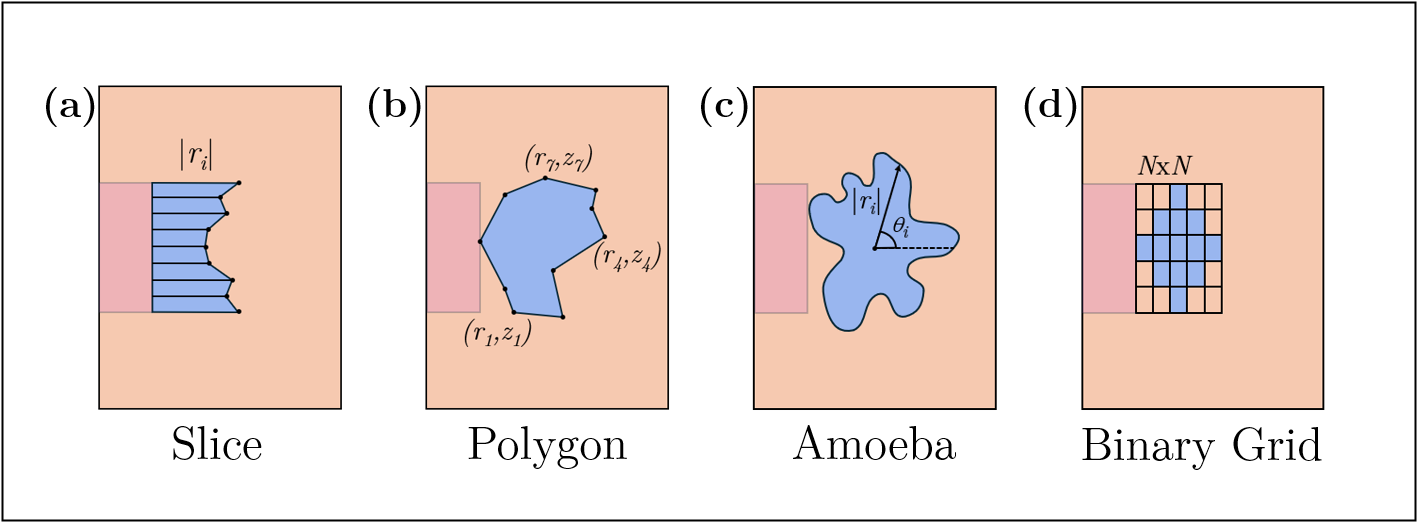
\includegraphics[width=0.9\textwidth]{figures/figure7.png}
  \caption{
    Visual comparison of four dielectric resonator modelling strategies. (a) The
    Slice method defines a shape using evenly spaced radial vectors of variable
    length $r_i$, projecting horizontally from a fixed vertical edge. (b) The
    Polygon method connects a series of coordinate points $(r_i,z_i)$ to form a
    closed, angular 2D shape. (c) The Amoeba method creates a smooth, continuous
    outline using radial vectors defined by length $r_i$ and angle $\theta_i$,
    giving rise to curved geometries. (d) The Binary Grid method divides the
    dielectric region into an $N\times N$ matrix of square domains, each
    representing either air or dielectric, allowing for flexible pixel-based
    geometry control.
  }
  \label{fig:figure7}
\end{figure}
